\documentclass[12pt]{article}
\usepackage[utf8]{inputenc}
\usepackage[frenchb]{babel}
\usepackage[T1]{fontenc}
\usepackage{authblk}
\usepackage{hyperref}
\usepackage{fancyhdr}
\usepackage{titling}
\usepackage{graphicx}
\usepackage{geometry}
\usepackage{enumitem}
\usepackage{microtype}
\usepackage[none]{hyphenat}
%\usepackage[toc]{glossaries}
%\makeglossaries
\usepackage{wrapfig}

\usepackage{perpage} %the perpage package
\MakePerPage{footnote} %the perpage package command

%\newacronym{REST}{REST}{transfert d'état représentationnel}


 \geometry{
 a4paper,
 total={169mm,240mm},
 left=16mm,
 top=20mm,
 }

\usepackage{listings} % For code coloration
\usepackage{color}
\usepackage[dvipsnames]{xcolor}


\definecolor{codegreen}{rgb}{0,0.6,0}
\definecolor{codegray}{rgb}{0.5,0.5,0.5}
\definecolor{codepurple}{rgb}{0.58,0,0.82}
\definecolor{backcolour}{rgb}{0.95,0.95,0.92}


\headheight = 15pt

\hypersetup{colorlinks = true,citecolor=black,filecolor=black,linkcolor=black,urlcolor=black}

\lstdefinestyle{s}{
  backgroundcolor=\color{backcolour},   commentstyle=\color{codegreen},
  keywordstyle=\color{NavyBlue},
  numberstyle=\tiny\color{codegray},
  stringstyle=\color{codepurple},
  basicstyle=\footnotesize,
  breakatwhitespace=false,
  breaklines=true,
  captionpos=b,
  keepspaces=true,
  numbers=left,
  numbersep=5pt,
  showspaces=false,
  showstringspaces=false,
  showtabs=false,
  tabsize=4
}


\lstset{style=s}
\lstset{literate=
  {á}{{\'a}}1 {é}{{\'e}}1 {í}{{\'i}}1 {ó}{{\'o}}1 {ú}{{\'u}}1
  {Á}{{\'A}}1 {É}{{\'E}}1 {Í}{{\'I}}1 {Ó}{{\'O}}1 {Ú}{{\'U}}1
  {à}{{\`a}}1 {è}{{\`e}}1 {ì}{{\`i}}1 {ò}{{\`o}}1 {ù}{{\`u}}1
  {À}{{\`A}}1 {È}{{\'E}}1 {Ì}{{\`I}}1 {Ò}{{\`O}}1 {Ù}{{\`U}}1
  {ä}{{\"a}}1 {ë}{{\"e}}1 {ï}{{\"i}}1 {ö}{{\"o}}1 {ü}{{\"u}}1
  {Ä}{{\"A}}1 {Ë}{{\"E}}1 {Ï}{{\"I}}1 {Ö}{{\"O}}1 {Ü}{{\"U}}1
  {â}{{\^a}}1 {ê}{{\^e}}1 {î}{{\^i}}1 {ô}{{\^o}}1 {û}{{\^u}}1
  {Â}{{\^A}}1 {Ê}{{\^E}}1 {Î}{{\^I}}1 {Ô}{{\^O}}1 {Û}{{\^U}}1
  {œ}{{\oe}}1 {Œ}{{\OE}}1 {æ}{{\ae}}1 {Æ}{{\AE}}1 {ß}{{\ss}}1
  {ű}{{\H{u}}}1 {Ű}{{\H{U}}}1 {ő}{{\H{o}}}1 {Ő}{{\H{O}}}1
  {ç}{{\c c}}1 {Ç}{{\c C}}1 {ø}{{\o}}1 {å}{{\r a}}1 {Å}{{\r A}}1
  {€}{{\EUR}}1 {£}{{\pounds}}1 {°}{{\no}}1
}

\pretitle{
  \begin{center}
  
\includegraphics[width=60mm,height=31mm]{img/univ.png}
  \qquad \qquad
  
\includegraphics[width=37mm,height=31mm]{img/iutNantes.jpg}\\[\bigskipamount]
}

\posttitle{
 \end{center}
}

\title{Back End marketing conversationnel\\
    \normalsize Technologies web côté serveur}
\date{\today}
\author{Paul Orhon\\
\small LP -- MiAR -- Université de Nantes }

\pagestyle{fancy}
\fancyhf{}
\rhead{Paul Orhon --- \small LP -- MiAR}
\lhead{Marketing conversationnel --- Technologies web côté serveur}
\rfoot{Page \thepage}
\lfoot{INSTITUT UNIVERSITAIRE DE TECHNOLOGIE - NANTES}


\begin{document}

\maketitle%page titre
\begin{figure}[h]
    \centering
    
\includegraphics[]{img/logo.png}
\end{figure}

\clearpage
\tableofcontents

\listoffigures


\clearpage

\section{Projet}
Dans le cadre du module de technologies web côté serveur, il a été demander de créer une partie du back end d’un marketing conversationnel.
\\

Pour cela il va falloir développer différent services pour pouvoirs mettre en place ce système.



\section{Contexte du projet}
\subsection{Objectifs}
L'objectif est donc de développer une partie du Back End d’un marketing conversationnel, en exposant les service avec une api REST.
\\

\begin{figure}[h]
    \centering
    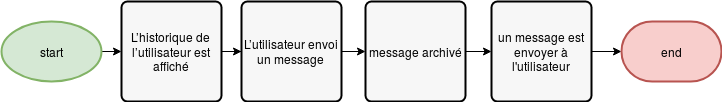
\includegraphics[width=\linewidth]{img/workflow_user.png}
    \caption{Workflow classique d'un utilisateur}
\end{figure}

La partie à développer est l'envoi des messages et les sauvegardes des données. Ces sauvegardes sont utilisé pour conserver les messages, qui seront daté, afin d'afficher l'historique à l'utilisateur et pouvoir effectuer des statistiques anonyme sur toute les conversation.
\\

Le projet doit être séparer en sous module, cela permettra de manipuler, modifier et diffuser plus facilement.


\subsection{Contraintes}
\begin{enumerate}
    \item Le projet est à réalisé seul.
    \item Le programme sera développé sur la plateforme Java.
    \begin{itemize}
        \item Il sera programmé en Java pour des raisons de connaissance.
    \end{itemize}
    \item Le rapport est à rendre le 23 novembre 2017 à 17h50.
    \item Le projet est à rendre le 5 décembre 2017 à 12h20.
    \item Le système doit sauvegarder les messages pour réaliser des statistiques et pour l'historique des utilisateurs.
    \item Le système doit être testé et testable sur le poste du développeur.
    \item Le couplage doit être lâche.
\end{enumerate}


\clearpage
\section{Les vues}
\subsection{Vue globale du projet}

\begin{figure}[h]
    \centering
    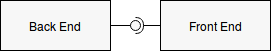
\includegraphics[]{img/Diagramme_sep_Back_Front.png}
    \caption{Diagramme de la séparation du Back / Front End}
    \label{fig:diag_back_front}
\end{figure}
Comme dit précédemment, seule le back end et son interface sera développer (partie en rouge de la figure \ref{fig:diag_back_front}).


\subsection{Vue logique du Back End}
Le back end sera diviser en plusieurs modules permettent ainsi de diviser les tâches, de réaliser un couplage lâche et de faciliter le maintien du système.

Cette représentation repose sur le \textit{domain-driven design} \footnote{\textit{domain-driven design}(DDD): en français \textit{conception pilotée par le domaine} est une approche de la conception de logiciel. Plus d'information: \url{https://en.wikipedia.org/wiki/Domain-driven_design}}.

\begin{figure}[h]
    \centering
    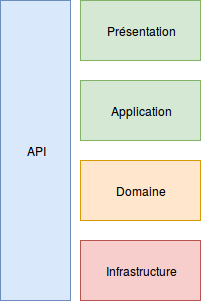
\includegraphics[]{img/Vue_logique_back.png}
    \caption{Diagramme de la vue logique du back end}
\end{figure}

Ici chaque couleur correspond à un module.


\begin{description}
    \item [Application] contient la \textbf{présentation} du fait de l'utilisation du framework \textit{Spring} qui permet une mise en place simple d'une api REST et donc de l'interface du back end. Sont rôle est de récupérer les requête arrivant à l'interface, de les envoyer au bon service et de répondre.
    \item [Domaine] correspond au \textit{services} de l'application. Contient aussi les interface, pressant  dans l'\textbf{API} et implémenté dans l'\textbf{infrastructure}, utile à ces services.
    \item [Infrastructure] correspond à l'implémentation des différentes \textbf{\textit{interfaces}} et \textbf{\textit{classe abstraites}} qui sont les factory. Il gère le stockage persistant des données.
    \item [API] contient les \textbf{\textit{classe}} communes aux modules. Cela permet notamment au \textbf{domaine} d'utiliser une classe et de laisser l'implémentation à l'\textbf{Infrastructure}.
\end{description}

\section{Implémentation}

\subsection{Les Services}
Le back end va donc proposer différant services.

\subsubsection{L'envoi de messages}
Un service proposera au client d'envoyer un message ver le serveur.
Ce message sera	transmis au personnes concerner. Il sera aussi sauvegarder. Cette sauvegarde est utile pour l'historique de conversation de l'utilisateur (cf. \ref{recup_histo}) et pour réaliser des statistique sur l'ensemble des demande.


\subsubsection{L'envoi de réponse}
Suite à l'envoi d'un message par un utilisateur, si il le peut, le serveur envoi un message sinon la personne concerner répond à la demande.\\
Pour le moment le serveur répondra avec un message générique, pour cause d'un manque de temps et de moyen.


\subsubsection{Récupérer l'historique} \label{recup_histo}
L'or de sa connections l'utilisateur peu récupérer son historique de conversation afin de reprend le fil de sa conversation.
\\
Si l'utilisateur na pas d'historique une liste vide luis est retourner.


% \subsection{Plateforme / Langage}

\subsection{Java}
Comme dit précédemment le programme sera développer pour la plateforme java et développer en java et plus précisément dans la version 8. Cela permet de faciliter le déploiement du programme.


\subsection{Librairie}

\subsubsection{Slf4j}
\textit{Slf4j}\footnote{\url{http://www.slf4j.org}} est une api de logging. Elle permet de loger les informations souhaiter à l'endroit souhaiter. Par exemple dans un fichier.

\subsubsection{Spring Boot} \label{SpringBoot}
Nous allons aussi utiliser \textit{Spring Boot}\footnote{\url{http://projects.spring.io/spring-boot}} en version 1.5.8 qui est un framework permettant de développer une application web avec une gestion simplifié des différents services mis en place et de leur présentation sous forme de service REST.

\subsubsection{Spring Boot Test}
\textit{Spring Boot Test}\footnote{\url{https://spring.io/guides/gs/spring-boot/\#_add_unit_tests}} est utiliser pour réaliser les tests de l'api REST. Nous l'utiliserons dans la même version que Spring Boot (cf. \ref{SpringBoot}).

\subsubsection{Junit}
Pour les test plus générale, nous allons utiliser \textit{junit}\footnote{\url{http://junit.org/junit4/}} en version 4.12, qui est un framework de test unitaire.



\subsection{Outils}
Pour ce projet nous utiliserons différant outils qui vont simplifier le développement.


\subsubsection{IntelliJ IDEA}
\textit{IntelliJ IDEA}\footnote{\url{https://www.jetbrains.com/idea/}} est l'IDE java qui est utiliser pour ce projet. Il va permettre de faciliter le développement grâce à ces différente options.


\subsubsection{Maven}
\textit{Maven}\footnote{\url{http://maven.apache.org/}} est un outil de gestion et d'automatisation de production des projets Java. Il va être utiles pour la séparation du programme en module, la gestion des dépendance et les build.

\subsubsection{MongoDB}
\textit{MongoDB}\footnote{\url{https://www.mongodb.com/what-is-mongodb}} est un système de gestion de base de données orientée documents, il est simple d'utilisation. Il va être utiliser pour sauvegarder les messages des utilisateur afin de leur retourner leur historique (cf. \ref{recup_histo}).

\subsubsection{GitHub}
\textit{GitHub}\footnote{\url{https://github.com/}} est un service de gestion de développement. Il va être utiliser pour gérée les versions du projet. Cela va aussi permettre le partage des sources sous licence MIT affin de récupérer le retour des utilisateurs et de leur amélioration.

\subsubsection{Travis-ci}
\textit{Travis-ci}\footnote{\url{https://travis-ci.org/}} est un outil d'intégration continue, qui permettre d'effectuer les build et les tests sous différent environnement UNIX. Il permet aussi de déployer les build.\\
Il est aussi possible d'utiliser \textit{AppVeyor} pour un environnement Windows.

\subsubsection{Codecov}
\textit{Codecov}\footnote{\url{https://codecov.io/gh}} est un outil permettant de regrouper, fusionner, archiver et comparer des rapports de couverture de code. Cela permet de trouver notamment les code mort.


\section{Conclusion}
Ce projet a donc pour but de développer le back end et l'interface d'un marketing conversationnel. Pour des raison de temps seul l'échange de messages et l'historique sera développer. Le projet sera réaliser en java. Différent outil serons utiliser pour faciliter le développement.

\begin{figure}[h]
    \centering
    
\includegraphics[]{img/logo.png}
    \caption{Logo}
\end{figure}



%\clearpage
%\printglossary[type=\acronymtype, title=Acronymes]

\end{document}
